\documentclass{beamer}
\usepackage[utf8x]{inputenc}
\usepackage[T2A]{fontenc}
\usepackage[english, russian]{babel}
\usepackage{graphicx}
\usepackage{listings}
\usepackage{ragged2e}

% Титульный слайд
\usetheme{Warsaw}
\begin{document}
\title{Краткое введение в язык DOT}
\author{Ершов Виталий РК6-72Б}
\institute{Московский государственный технический университет имени Н. Э. Баумана}
\date{Москва, 2021} 
\frame{\titlepage}

% Слайд 2
\begin{frame}{Что такое язык DOT?}
	DOT - это язык описания графов.
	\newline
	\newline
	Граф, описанный на языке DOT, обычно представляет собой текстовый файл с расширением .gv или .dot в понятном для человека и обрабатывающей программы формате.
	\begin{figure}[h]
	\begin{minipage}[h]{0.49\linewidth}
	\center{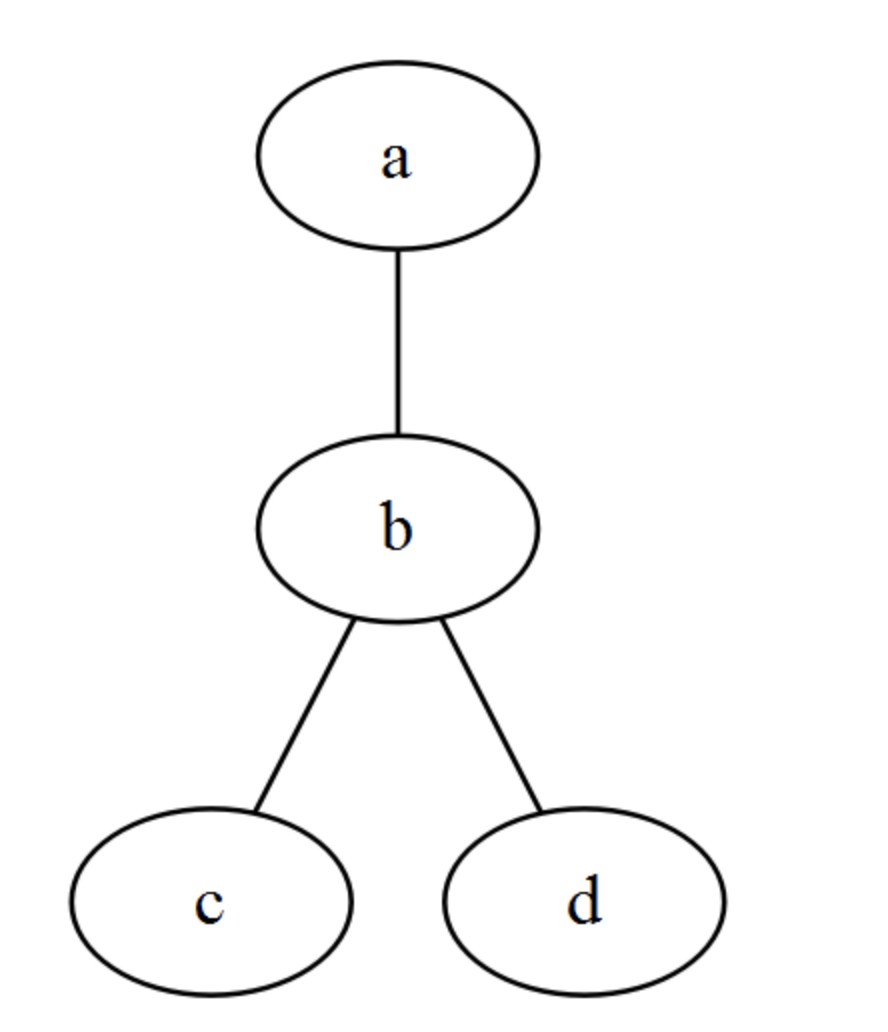
\includegraphics[width=0.5\linewidth]{images/image1.png} \\ Неориентированный граф}
	\end{minipage}
	\hfill
	\begin{minipage}[h]{0.49\linewidth}
	\center{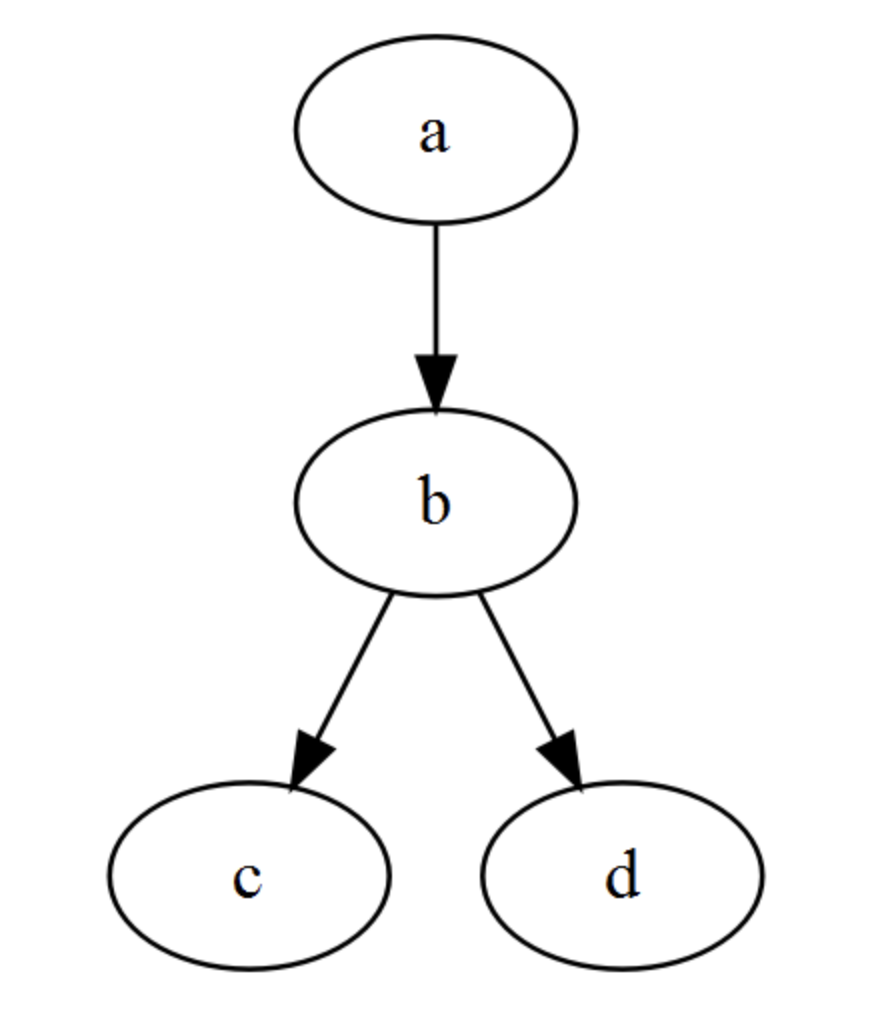
\includegraphics[width=0.5\linewidth]{images/image2.png} \\ Ориентированный граф}
	\end{minipage}
	\label{ris:image1}
	\end{figure}
\end{frame}

\begin{frame}[fragile]{Вызов программ}
	Для вызова программ написанных с использованием языка DOT используется следующая команда:
	\newline
	\newline
	\begin{minipage}{0.9\textwidth}
		\begin{verbatim}
			dot -Tpng input.dot -o graph.png
		\end{verbatim}
	\end{minipage}
	\newline
	\newline
	Для получения изображения графа в формате .png мы используем флаг \color{red}-Tpng\color{black}, далее задаем путь к файлу с описанным графом и затем, с помощью флага \color{red}-o\color{black}, мы задаем файл для вывода результата. Таким образом, в результате выполнения этой команды мы вызовем программу input.dot и получим изображение графа в файле graph.png.
\end{frame}

% Слайд 3
\begin{frame}[fragile]{Введение в синтаксис языка DOT}
	Любое описание графа с помощью языка DOT начинается с определения типа графа. Для неориентированных графов описание начинается с ключевого слова \color{red}graph\color{black}, а для ориентированных с ключевого слова \color{red}diagraph\color{black}.
	\newline
	\newline
	\begin{minipage}{0.5\textwidth}
		\raggedrightСтруктура неориентированного графа приведенного на этом слайде
		\begin{verbatim}
				graph G {
				    a -- b;
				    a -- d -- c;
				    d -- e;
				}
		\end{verbatim}
	\end{minipage}
	\hfill
	\begin{minipage}{0.45\textwidth}
	 	\center{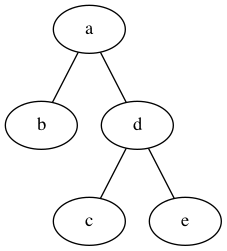
\includegraphics[width=0.7\linewidth]{images/image3.png}}
	\end{minipage}
\end{frame} 

 % Слайд 4
\begin{frame}[fragile]{Введение в синтаксис языка DOT}
	\begin{minipage}{0.5\textwidth}
		\raggedrightСтруктура ориентированного графа приведенного на этом слайде
		\begin{verbatim}
				digraph G {
				    a -> b;
				    a -> d -> c;
				    d -> e;
				}
		\end{verbatim}
	\end{minipage}
	\hfill
	\begin{minipage}{0.45\textwidth}
	 	\center{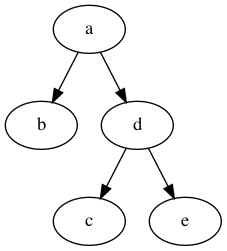
\includegraphics[width=0.7\linewidth]{images/image4.png}}
	\end{minipage}
	\newline
	\newline
	\color{red}Заметим\color{black}, что в ориентированном графе для задания ребра между двумя узлами используется \color{red}'->'\color{black}, в то время, как в неориентированном \color{red}'--'\color{black}.
\end{frame}  

% Слайд 5
\begin{frame}[fragile]{Стилизация элементов}
	Язык DOT позволяет стилизировать элементы графа, таким образом, можно изменить форму вершины и назначить ей метку (по умолчанию метка - название вершины). Также можно изменять цвета и стиль ребер, например сделать ребро пунктирной линией. Список всех возможностей по стилизации графов приведен на официальном сайте https://graphviz.org/
	\newline
	\newline
	\begin{minipage}{0.5\textwidth}
		\begin{verbatim}
				digraph G {
					node[shape=diamond];
					a [label="Node A"];
					b [shape=circle];
					c [color=lightblue];
					a -> b;
					a -> c [style=dotted, color=red];
				}
		\end{verbatim}
	\end{minipage}
	\hfill
	\begin{minipage}{0.45\textwidth}
	 	\center{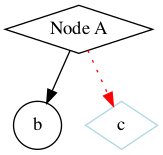
\includegraphics[width=0.7\linewidth]{images/image5.png}}
	\end{minipage}
\end{frame}             

% Слайд 6
\begin{frame}[fragile]{Расположение меток}
	С помощью свойства \color{red}xlabel \color{black}можно расположить метку рядом с узлом, а не внутри него. Иногда это свойство может очень полезно, например, мы хотим описать какие-то свойства вершины и логично это сделять рядом, а не внутри.
	\newline
	\newline
	\begin{minipage}{0.5\textwidth}
		\begin{verbatim}
				digraph G {
					rankdir="LR";
					a [xlabel="Vertex A"];
					a -> b;
					d [xlabel="Vertex D"];
					a -> c -> d;
				}
		\end{verbatim}
	\end{minipage}
	\hfill
	\begin{minipage}{0.45\textwidth}
	 	\center{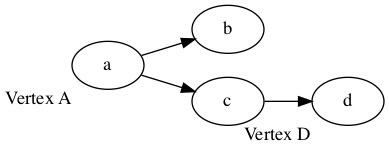
\includegraphics[width=0.9\linewidth]{images/image6.png}}
	\end{minipage}
\end{frame}

% Слайд 7
\begin{frame}[fragile]{Направление графа}
	На прошлом слайде, в описание графа было добавлено свойство \color{red}rankdir \color{black}. C помощью данного свойства мы можем установить направление графа. Таким образом. Можно задать направление ''LR'' - граф будет строиться слева направо, ''BT'' - граф будет строиться снизу вверх.
	\newline
	\newline
	\begin{minipage}{0.5\textwidth}
		\begin{verbatim}
				digraph G {
					rankdir = "BT";
					a -> b -> c;
				}
		\end{verbatim}
	\end{minipage}
	\hfill
	\begin{minipage}{0.45\textwidth}
	 	\center{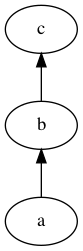
\includegraphics[height=0.9\linewidth]{images/image7.png}}
	\end{minipage}
\end{frame}      

% Слайд 8
\begin{frame}[fragile]{Использование HTML в метках}
	В языке DOT при задании меток можно использовать язык разметки HTML, так в примере приведенном ниже, используя HTML, мы сделали текст метки жирным и курсивным.
	\newline
	\newline
	\begin{minipage}{0.5\textwidth}
		\begin{verbatim}
				digraph G {
					rankdir = "LR";
					1 -> 3;
					2 [label=<<b><i>2</i></b>>];
					1 -> 2;
				}
		\end{verbatim}
	\end{minipage}
	\hfill
	\begin{minipage}{0.45\textwidth}
	 	\center{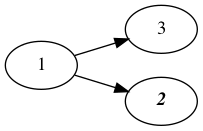
\includegraphics[height=0.6\linewidth]{images/image8.png}}
	\end{minipage}
\end{frame}

% Слайд 9
\begin{frame}[fragile]{Расположение узлов графа}
	Для того, чтобы изменить распложение узлов графа по умолчанию им задают разный вес. Таким образом, в примере приведенном ниже, часть ребер имеет больший вес, следовательно они будут расположены вдоль одной прямой, а ребра с меньшим весом будут располагаться ниже.
	\newline
	\newline
	\begin{minipage}{0.4\textwidth}
		\begin{verbatim}
				digraph G {
					rankdir = "LR";
					node[width=0.15,
					     height=0.15,
					     shape=point];
					edge[weight=2];
					1 -> 2 -> 3 -> 4 -> 5;
					edge[weight=1];
					2 -> 6 -> 7;
				}
		\end{verbatim}
	\end{minipage}
	\hfill
	\begin{minipage}{0.55\textwidth}
	 	\center{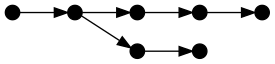
\includegraphics[height=0.25\linewidth]{images/image9.png}}
	\end{minipage}
\end{frame}

% Слайд 10
\begin{frame}[fragile]{Заключение}
	\begin{minipage}{0.5\textwidth}
		В течение презентации мы ознакомились с языком DOT с помощью которого можно визуализировать графы. Показанное в этой презентации - это лишь малая доля возможностей языка. При более детальном изучении языка открывается широкий спектр возможностей для описания графов разной степени сложности.
	\end{minipage}
	\hfill
	\begin{minipage}{0.4\textwidth}
	 	\center{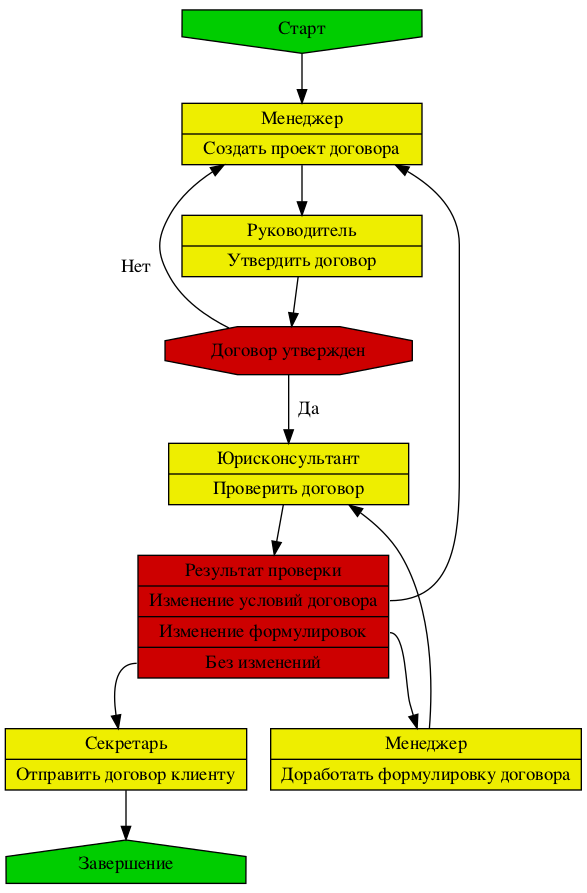
\includegraphics[height=1.7\linewidth]{images/image10.png}}
	\end{minipage}
\end{frame}          

\end{document}